\documentclass{sigchi}

% Use this section to set the ACM copyright statement (e.g. for
% preprints).  Consult the conference website for the camera-ready
% copyright statement.

% Copyright

%\setcopyright{acmcopyright}
%\setcopyright{rightsretained}
%\setcopyright{usgov}
%\setcopyright{usgovmixed}
%\setcopyright{cagov}
%\setcopyright{cagovmixed}
% DOI
\doi{https://doi.org/10.1145/3313831.XXXXXXX}
% ISBN
\isbn{978-1-4503-6708-0/20/04}
%Conference
\conferenceinfo{CHI'20,}{April  25--30, 2020, Honolulu, HI, USA}
%Price
\acmPrice{\$15.00}

% Use this command to override the default ACM copyright statement
% (e.g. for preprints).  Consult the conference website for the
% camera-ready copyright statement.

%% HOW TO OVERRIDE THE DEFAULT COPYRIGHT STRIP --
%% Please note you need to make sure the copy for your specific
%% license is used here!
% \toappear{
% Permission to make digital or hard copies of all or part of this work
% for personal or classroom use is granted without fee provided that
% copies are not made or distributed for profit or commercial advantage
% and that copies bear this notice and the full citation on the first
% page. Copyrights for components of this work owned by others than ACM
% must be honored. Abstracting with credit is permitted. To copy
% otherwise, or republish, to post on servers or to redistribute to
% lists, requires prior specific permission and/or a fee. Request
% permissions from \href{mailto:Permissions@acm.org}{Permissions@acm.org}. \\
% \emph{CHI '16},  May 07--12, 2016, San Jose, CA, USA \\
% ACM xxx-x-xxxx-xxxx-x/xx/xx\ldots \$15.00 \\
% DOI: \url{http://dx.doi.org/xx.xxxx/xxxxxxx.xxxxxxx}
% }
\toappear{}

% Arabic page numbers for submission.  Remove this line to eliminate
% page numbers for the camera ready copy
% \pagenumbering{arabic}

% Load basic packages
\usepackage{balance}       % to better equalize the last page
\usepackage{graphics}      % for EPS, load graphicx instead 
\usepackage[T1]{fontenc}   % for umlauts and other diaeresis
\usepackage{txfonts}
\usepackage{mathptmx}
\usepackage[pdflang={en-US},pdftex]{hyperref}
\usepackage{color}
\usepackage{booktabs}
\usepackage{textcomp}

% Some optional stuff you might like/need.
\usepackage{microtype}        % Improved Tracking and Kerning
% \usepackage[all]{hypcap}    % Fixes bug in hyperref caption linking
\usepackage{ccicons}          % Cite your images correctly!
% \usepackage[utf8]{inputenc} % for a UTF8 editor only

% If you want to use todo notes, marginpars etc. during creation of
% your draft document, you have to enable the "chi_draft" option for
% the document class. To do this, change the very first line to:
% "\documentclass[chi_draft]{sigchi}". You can then place todo notes
% by using the "\todo{...}"  command. Make sure to disable the draft
% option again before submitting your final document.
\usepackage{todonotes}

% Paper metadata (use plain text, for PDF inclusion and later
% re-using, if desired).  Use \emtpyauthor when submitting for review
% so you remain anonymous.
\def\plaintitle{Preventing Bias in Machine Learning by using Bias Aware Algorithms: An Empirical Experimental Study - Full Report}
\def\plainauthor{First Author, Second Author, Third Author,
  Fourth Author, Fifth Author, Sixth Author}
\def\emptyauthor{}
\def\plainkeywords{Authors' choice; of terms; separated; by
  semicolons; include commas, within terms only; this section is required.}
\def\plaingeneralterms{Documentation, Standardization}

% llt: Define a global style for URLs, rather that the default one
\makeatletter
\def\url@leostyle{%
  \@ifundefined{selectfont}{
    \def\UrlFont{\sf}
  }{
    \def\UrlFont{\small\bf\ttfamily}
  }}
\makeatother
\urlstyle{leo}

% To make various LaTeX processors do the right thing with page size.
\def\pprw{8.5in}
\def\pprh{12in}
\special{papersize=\pprw,\pprh}
\setlength{\paperwidth}{\pprw}
\setlength{\paperheight}{\pprh}
\setlength{\pdfpagewidth}{\pprw}
\setlength{\pdfpageheight}{\pprh}

% Make sure hyperref comes last of your loaded packages, to give it a
% fighting chance of not being over-written, since its job is to
% redefine many LaTeX commands.
\definecolor{linkColor}{RGB}{6,125,233}
\hypersetup{%
  pdftitle={\plaintitle},
% Use \plainauthor for final version.
%  pdfauthor={\plainauthor},
  pdfauthor={\emptyauthor},
  pdfkeywords={\plainkeywords},
  pdfdisplaydoctitle=true, % For Accessibility
  bookmarksnumbered,
  pdfstartview={FitH},
  colorlinks,
  citecolor=black,
  filecolor=black,
  linkcolor=black,
  urlcolor=linkColor,
  breaklinks=true,
  hypertexnames=false
}

% create a shortcut to typeset table headings
% \newcommand\tabhead[1]{\small\textbf{#1}}

% End of preamble. Here it comes the document.
\begin{document}

\title{\plaintitle}

\numberofauthors{3}
\author{%
  \alignauthor{Andy Gray\\
    \affaddr{445348}\\
    \email{445348@swansea.ac.uk}}
}

\maketitle

\section{Introduction}

[Project Discription]\\
We aim to remove the potential gender bias in a suggested pay to an employee from data with a clear gender bias within the dataset. 

[Motivation]\\
\textbf{In 2018, women, no matter their background, on average earned just 82 cents for every \$1 earned by men \cite{1}. ML requires vast amounts of past data to inform future events, with AI and machine learning being the key driver behind many decisions. However, with there being a well-known gap between a person's gender and their pay, the ML models will only learn this and use this as a factor in their decisions making. Therefore, to stop this from happening, a system needs to be put into place to remove this process's bias.} 

\textbf{Using fairness techniques at preprocessing stages \cite{3} of supervised learning, we will aim to remove the bias of someone's gender from a suggested pay salary for an individual. }

[Summary of existing lit]

[Problems with lit]

[Project Spec]

[Result findings]

[Overview]

\section{Background \& Literature Review}


\subsection{Study Design}
	Our study is around the topic of bias in algorithms and looking at ways to remove these biases. The study will be looking at ways to detect the bias, measure it and then reduce it. Our study got carried out in a manner that follows an empirical experimental study method. 

	Our study has looked into ways to identify bias within a dataset and then look at ways to remove this bias, ensuring that protected characteristics, in our case gender, do not impact or impede a person's proposed suggested salary.  

	We aimed to try and find out if there was first any bias within the dataset. We did this by first plotting out the dataset based on the characteristic of male and female. We initially created a model that would truthfully represent the gender bias within the model's predictions.

	To achieve removing the bias, we extracted the prediction-specific interactions. By getting the interactions, we could cancel out their effect and the influence driven by the gender variable. We then re-calculate our predictions, which immediately shows the removal of any sign of prejudice within the dataset. Additionally, the model conscientiously captures the variation driven by the employee's years of employment and career path. 

	This bias-aware approach to modelling can be applied to other forms of input types, with a similar approach being used by Google \cite{google_ref}

\subsection{Libraries}
	We used Python 3 \cite{python} to create the empirical experiment. Additional libraries used were Pandas \cite{pandas} to allow us to load in the data and wrangle the data frames. Seaborn \cite{seaborn} was also used to visualise the data. XGBoost \cite{xgboost} to create the model and extract the critical interactions from within the model. 

\subsection{Dataset and Data Preprocessing}
	Synthetic dataset based around two job types -> why because was hard to find data set that does not provide "just an overview". 

pandas.get\_dummies


\section{Results \& Analysis}



Unmodified dataset:
\begin{figure}[h]
	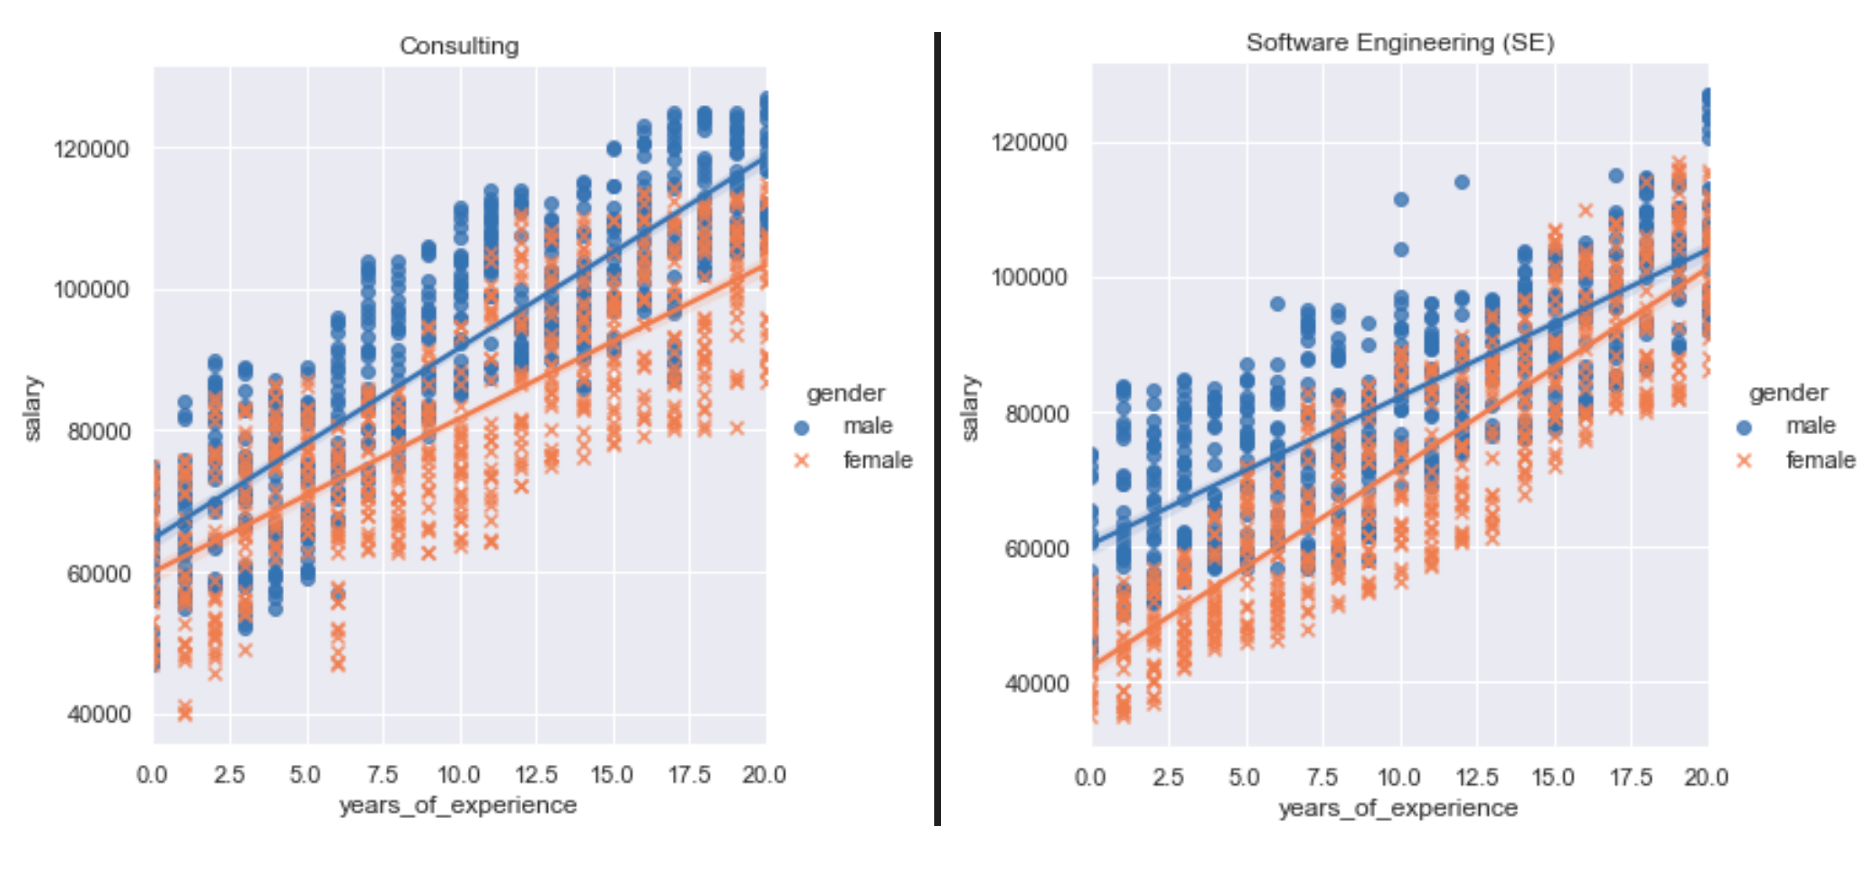
\includegraphics[width=8cm]{original_data.png}
	\centering
\end{figure}

\begin{figure}[h]
	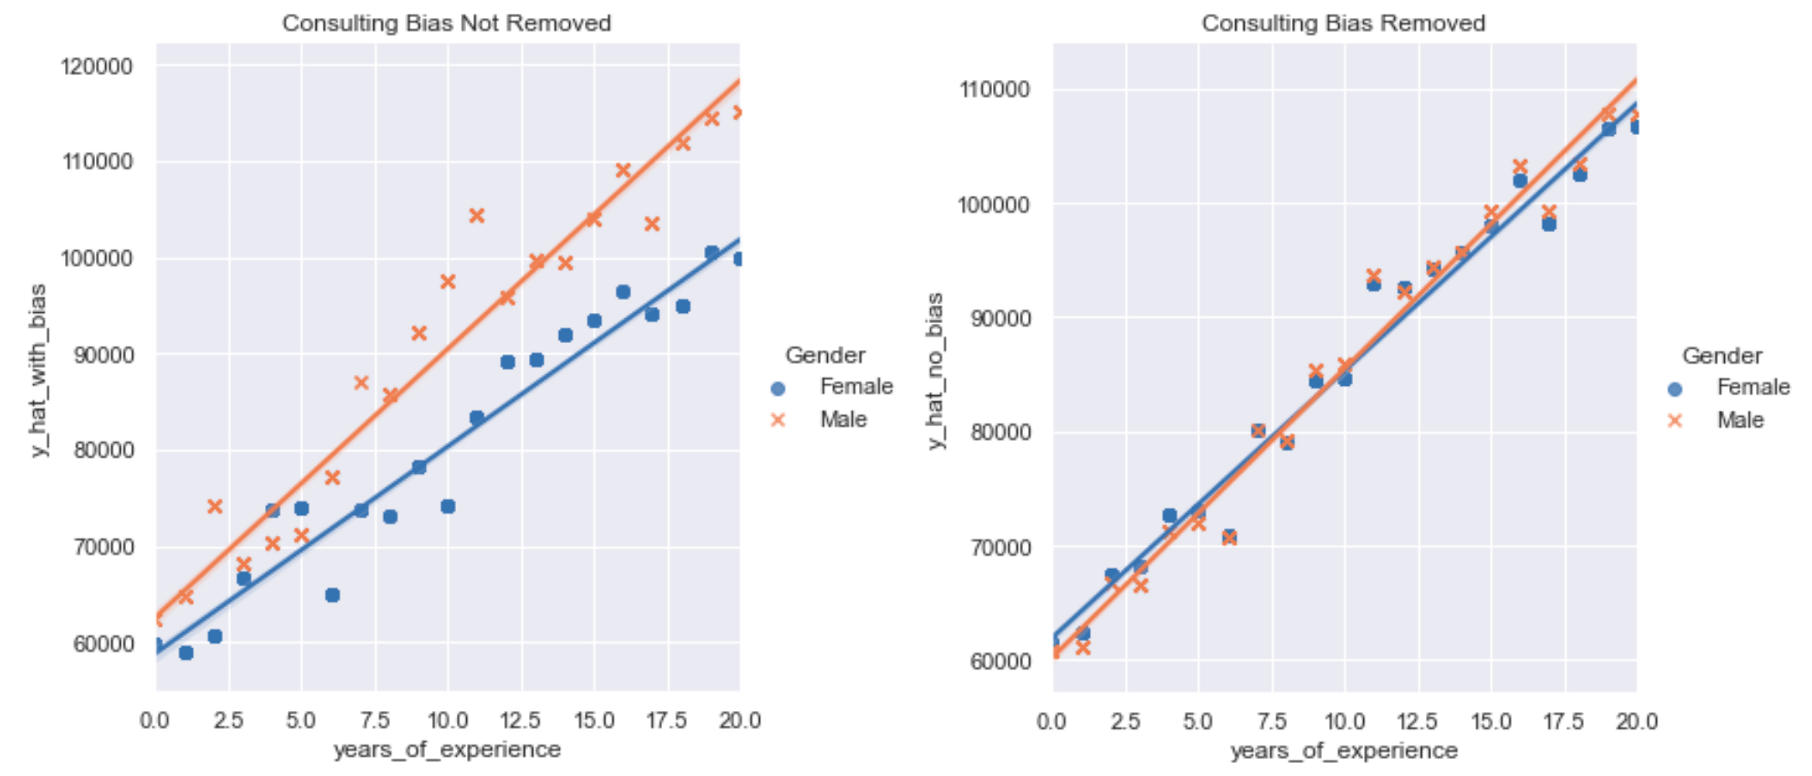
\includegraphics[width=8cm]{consulting_comparison.png}
	\centering
\end{figure}

\begin{figure}[h]
	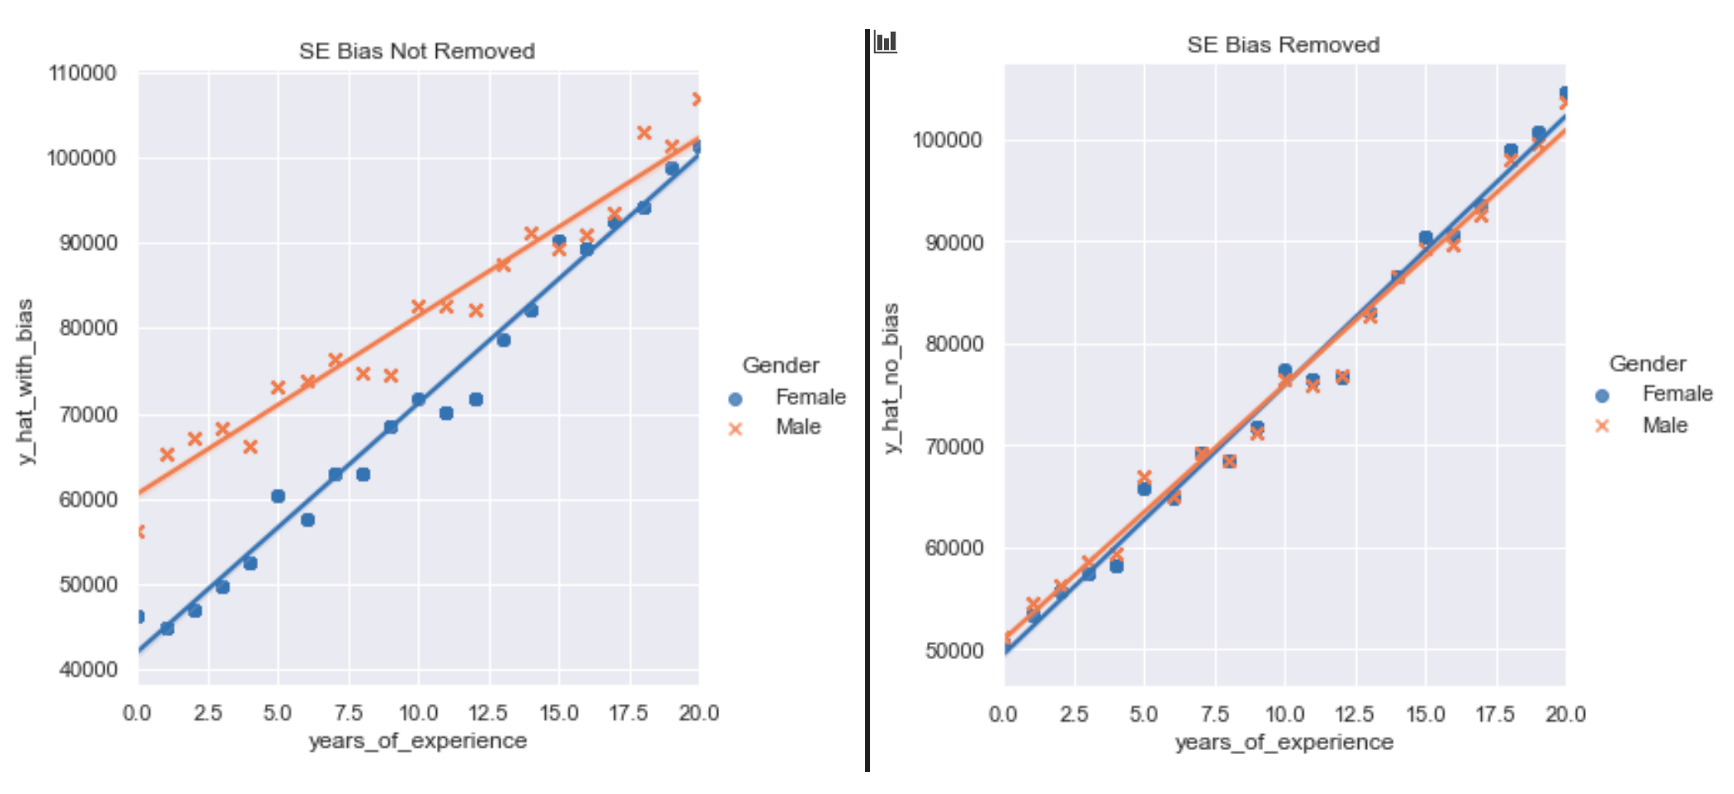
\includegraphics[width=8cm]{se_comparison.png}
	\centering
\end{figure}



\section{Discussion \& Conclusion}
	[discussion]
	
	[conclusion] \\
	\textbf{I would like to point out from the outset that there is no question that this approach will lead to a decrease in model performance on your validation data. In our contrived example, the RMSPE is 12\% for predictions that encode bias and 14\% for predictions where we removed the gender contribution. Nonetheless, this decrease in performance is acceptable and encouraged in many settings. After all, the purpose of your models is not only to make good predictions but to also allow you to identify ways to pull levers, such as modify user behavior on your website or prevent harmful things from happening when diagnosing a disease. Hence, if you want to build a model that is not prejudiced by your data, you can’t go wrong with letting the model first measure the amount of prejudice and then resetting all the bias contributing factors to zero.}


\newpage
% BALANCE COLUMNS
\balance{}
% REFERENCES FORMAT
% References must be the same font size as other body text.
\bibliographystyle{SIGCHI-Reference-Format}
\bibliography{sample}

\end{document}

%%% Local Variables:
%%% mode: latex
%%% TeX-master: t
%%% End:
